
\subsection{Representation theory - case $l=0$}

Here we investigate the maps between standard modules at special values of $\alpha$. 
Recall that for $l=-1$ we presented corresponding data in Fig.\ref{fig:gramdets03}.
Perhaps the first thing to do here is to find an embedding of the Rollet graph at $l=0$ in the plane (of the page) so that data can be presented in as uncluttered a way as possible. One possibility is:
\newcommand{\ver}[1]{{\!\!\!\!\!\!\begin{array}{c} { } \\ \bullet \\ \!\!\!\! \scriptsize{#1} \!\!\!\! \end{array}\!\!\!\!\!\!}}
\[
\hspace{-2.1cm} 
\xymatrix{
   &&&&&& \;\bullet_0 \ar@{-}[d] \\
\ver{(7,\!(2))} \ar@{-}[r] & 
\ver{(6,\!(2))} \ar@{-}[r] & 
\ver{(5,\!(2))} \ar@{-}[r] & 
\ver{(4,\!(2))} \ar@{-}[r] & 
\ver{(3,\!(2))} \ar@{-}[r] & 
\ver{(2,\!(2))} \ar@{-}[r] & 
\bullet_1 \ar@{-}[r] & 
\ver{(2,\!(1^2))} \ar@{-}[r] & 
\ver{(3,\!(1^2))} \ar@{-}[r] & 
\ver{(4,\!(1^2))} \ar@{-}[r] & 
\bullet \ar@{-}[r] & 
\bullet \ar@{-}[r] & 
\ver{(7,\!(1^2))} & 
}
\]



\subsubsection{Subcase $\alpha =1$}  \label{ss:alph1}

%\ppm{[to add - nice Loewy example...]}
Observe from Fig.\ref{fig:Bratelli-l0-gramdets} (say) that 
the first singular gram matrix here is for  $\Delta^{3}_{(3,(1))}$. 
The only possible maps in are from the one-dimensional modules 
$\Delta^{3}_{(3,(3))}$ and/or $\Delta^{3}_{(3,(1^3))}$. 
Thus we are looking for subspaces of the form:

%\newcommand{\rb}[1]{\raisebox{.85cm}{$\; #1 \;$}}
\newcommand{\IU}{
\raisebox{-.32cm}{
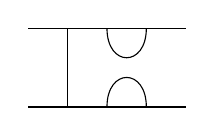
\begin{tikzpicture}
     \draw (0,0) -- (2,0) ;
     \draw (.5,0) -- (.5,-1);
     \draw (1,0) .. controls (1,-.5) and (1.5,-.5) .. (1.5,0) ;
     \draw (1,-1) .. controls (1,-.5) and (1.5,-.5) .. (1.5,-1) ;
 \draw (0,-1) -- (2,-1);
 \end{tikzpicture}
}}
\newcommand{\UI}{
\raisebox{-.32cm}{
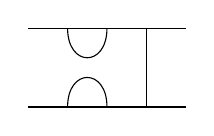
\begin{tikzpicture}
     \draw (0,0) -- (2,0) ;
     \draw (1.5,0) -- (1.5,-1);
     \draw (.5,0) .. controls (.5,-.5) and (1,-.5) .. (1,0) ;
     \draw (.5,-1) .. controls (.5,-.5) and (1,-.5) .. (1,-1) ;
 \draw (0,-1) -- (2,-1);
 \end{tikzpicture}
}}
\newcommand{\SigI}{
\raisebox{-.32cm}{
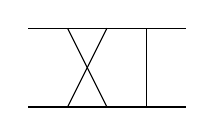
\begin{tikzpicture}
     \draw (0,0) -- (2,0) ;
     \draw (1.5,0) -- (1.5,-1);
     \draw (.5,0) -- (1,-1) ;
     \draw (.5,-1) -- (1,0) ;
 \draw (0,-1) -- (2,-1);
 \end{tikzpicture}
}}

\[ 
\rb{c\;} \begin{tikzpicture}
     \draw (0,0) -- (2,0) ;
     \draw (.5,0) -- (.5,-1);
     \draw (1,0) .. controls (1,-.5) and (1.5,-.5) .. (1.5,0) ;
 \end{tikzpicture}
 \rb{+\;b\;} \begin{tikzpicture}
     \draw (0,0) -- (2,0) ;
     \draw (1,0) -- (1,-1);
     \draw (.5,0) .. controls (.5,-.5) and (1.5,-.5) .. (1.5,0) ;
 \end{tikzpicture}
 \rb{+\;a\;} \begin{tikzpicture}
     \draw (0,0) -- (2,0) ;
     \draw (1.5,0) -- (1.5,-1);
     \draw (.5,0) .. controls (.5,-.5) and (1.0,-.5) .. (1,0) ;
 \end{tikzpicture}
\]
\medskip \medskip 

%\newcommand{\xx}{\alpha}

\noindent 
The action of 
\[
\UI \;\;\;\mbox{ and } \;\;\;  \IU 
\]
must be by 0, so in general 
$\xx a+b+c=0$ and $a+b+\xx c=0$. 
The action of the first elementary transposition
\[
\SigI  
\]
must be by 1 or -1, yielding $b=c$ and $a+2b=0$ in the + case; and $a=0$ and $b=-c$ in the - case, when $\xx=1$. Hence 1d solution spaces. 
(Note that here there is no second elementary transposition! If there were, the system would change radically.)
Thus we see that both one-dimensional $\Delta$-modules are submodules. 
By globalisation this means that we have 
\[
\Delta^{n}_{(3,(2))} \oplus \Delta^{n}_{(3,1^2)} \; \rightarrow\; \Delta^{n}_{(1,(1))}
\]
for all odd $n$, with both summands having nonzero image. 
We draw this as
\[
\hspace{-2.1cm} 
\xymatrix{
   &&&&&& \;\bullet_0 \ar@{-}[d] \\
\ver{(7,\!(2))} \ar@{-}[r] & 
\ver{(6,\!(2))} \ar@{-}[r] & 
\ver{(5,\!(2))} \ar@{-}[r] & 
\ver{(4,\!(2))} \ar@{-}[r]  & 
\ver{(3,\!(2))} \ar@{-}[r] \ar@[red]@/^1.3pc/[rr] & 
\ver{(2,\!(2))} \ar@{-}[r] & 
\bullet_1 \ar@{-}[r] & 
\ver{(2,\!(1^2))} \ar@{-}[r] & 
\ver{(3,\!(1^2))} \ar@{-}[r] \ar@[red]@/_1.3pc/[ll] & 
\ver{(4,\!(1^2))} \ar@{-}[r] & 
\bullet \ar@{-}[r] & 
\bullet \ar@{-}[r] & 
\ver{(7,\!(1^2))} & 
}
\] 

Looking at $n=4$ we see that by Frobenius reciprocity, 
with $A = \Delta^{n-1}_{(3,\lambda)}$ ($\lambda = (2), (1^2)$) and 
$B=\Delta^{n}_{(0,0)}$ in (\ref{eq:FR}), 
we have 
\[
\Delta^{n}_{(4,(2))} \oplus \Delta^{n}_{(4,1^2)} \; \rightarrow\; \Delta^{n}_{(0,(0))}
\]
On the other hand with $A=\Delta^{n-1}_{(3,(2))}$ and $B=\Delta^{n}_{(2,(1^2))}$ we have
\[
\hom(\Delta^{n}_{(4,(2))} \oplus \Delta^{n}_{(2,(2))} , \Delta^{n}_{(2,(1^2))} ) 
 \cong  
\hom(\Delta^{n-1}_{(3,(2))} , \Delta^{n-1}_{(3,(1^2))} + \Delta^{n-1}_{(1,(1))}) 
\]
The sum on the right is non-split, but both factors have $ \Delta^{n-1}_{(3,(2))} $ in the socle, so  the dimension on the right is at least 1. 
And hence also on the left - and by globalisation there is no map from 
$ \Delta^{n}_{(2,(2))}$ to $\Delta^{n}_{(2,(1^2))} $. So we deduce:
\[
\Delta^{n}_{(4,(2))}  \rightarrow   \Delta^{n}_{(2,(1^2))}
\]
(It is worth thinking about other choices for $A$ and $B$!... .) 
And similarly for ... by symmetry. 
Altogether that is:  % \ppm{[unfinished pic!!...]}:
\[
\hspace{-2.1cm} 
\xymatrix{
   &&&&&& \;\bullet_0 \ar@{-}[d] \\
\ver{(7,\!(2))} \ar@{-}[r] & 
\ver{(6,\!(2))} \ar@{-}[r] & 
\ver{(5,\!(2))} \ar@{-}[r] & 
\ver{(4,\!(2))} \ar@{-}[r] \ar@[red]@/^1.3pc/[rrru] \ar@[red]@/^1.9863pc/[rrrr] & 
\ver{(3,\!(2))} \ar@{-}[r] \ar@[red]@/^1.3pc/[rr] & 
\ver{(2,\!(2))} \ar@{-}[r] & 
\bullet_1 \ar@{-}[r] & 
\ver{(2,\!(1^2))} \ar@{-}[r] & 
\ver{(3,\!(1^2))} \ar@{-}[r] \ar@[red]@/_1.3pc/[ll] & 
\ver{(4,\!(1^2))} \ar@{-}[r] \ar@[red]@/_1.3pc/[lllu] \ar@[red]@/_1.93pc/[llll] & 
\bullet \ar@{-}[r] & 
\bullet \ar@{-}[r] & 
\ver{(7,\!(1^2))} & 
}
\] 

Notice that this is consistent with the gram matrix results as in Fig.\ref{fig:Bratelli-l0-gramdets}. 
In particular there is not a morphism from $(4,(2)) \rightarrow (2,(2))$ 
(in the obvious shorthand); nor the symmetry image version. 

Passing on to $n=5$ we see, taking $A=(4,(2))$ and $B=(3,(1^2))$ that 
\[
\hom(\Delta^{n}_{(5,(2))} \oplus \Delta^{n}_{(3,(2))} , \Delta^{n}_{(3,(1^2))} ) 
 \cong  
\hom(\Delta^{n-1}_{(4,(2))} , \Delta^{n-1}_{(2,(1^2))} + \Delta^{n-1}_{(4,(1^2))}) 
\]
Obviously there is a map $(4,(2))\rightarrow (2,(1^2))$, so dim-hom $\geq 1$ on the right unless the $(4,(1^2))$ is glued under - but this would imply a map that we 
noted above  %know 
is not there. Thus dim-hom on the left is nonzero. This forces 
$(5,(2))\rightarrow (3,(1^2))$; and its symmetry image. 
Altogether: 
\[
\hspace{-2.1cm} 
\xymatrix{
   &&&&&& \;\bullet_0 \ar@{-}[d] \\
\ver{(7,\!(2))} \ar@{-}[r] & 
\ver{(6,\!(2))} \ar@{-}[r] & 
\ver{(5,\!(2))} \ar@{-}[r] \ar@[green]@/^2.963pc/[rrrrrr] & 
\ver{(4,\!(2))} \ar@{-}[r] \ar@[red]@/^1.3pc/[rrru] \ar@[red]@/^1.9863pc/[rrrr] & 
\ver{(3,\!(2))} \ar@{-}[r] \ar@[red]@/^1.3pc/[rr] & 
\ver{(2,\!(2))} \ar@{-}[r] & 
\bullet_1 \ar@{-}[r] & 
\ver{(2,\!(1^2))} \ar@{-}[r] & 
\ver{(3,\!(1^2))} \ar@{-}[r] \ar@[red]@/_1.3pc/[ll] & 
\ver{(4,\!(1^2))} \ar@{-}[r] \ar@[red]@/_1.3pc/[lllu] \ar@[red]@/_1.93pc/[llll] & 
\bullet \ar@{-}[r] \ar@[green]@/_3.093pc/[llllll] & 
\bullet \ar@{-}[r] & 
\ver{(7,\!(1^2))} & 
}
\] 
Here there are the possibilities of composite maps:
\[
(5,(2)) \rightarrow (3,(1^2)) \rightarrow (1,(1)) 
\]
and symmetry image. Recall that in the $l=-1$ case all composite maps are zero 
(see \cite[Ch.6]{Martin91}).  
However here we deduce from the gram determinant that 
$ (3,(1^2)) \hookrightarrow (1,(1)) $, and hence the composite is non-zero. 

\subsubsection{Subcase  $(\alpha^2 + \alpha -4)=0$}

\mdef  
Let us have a look at $\alpha$ such that $(\alpha^2 + \alpha -4)=0$. 
Observe from Fig.\ref{fig:Bratelli-l0-gramdets} (say) that 
the first singular gram matrix is for  $\Delta^{4}_{(2,(2))}$. 
By globalisation the only possible maps in are from 
$\Delta^{4}_{(4,(2))}$ or from $\Delta^{4}_{(4,(1^2))}$. 
It is easy to check 
(see e.g. \S\ref{ss:bootcase0})
that there is no  $\Delta^4_{(4,(1^2))}$ subspace
(unless $\alpha=1$), 
so the subspace is $\Delta^4_{(4,(2))}$ here. 
%We can work out which by a little linear algebra. But let us keep going for now. 

By globalisation this means that we have module morphisms 
\beq \label{eq:morphismto22} 
\Delta^n_{(4,(2))}  \rightarrow \Delta^n_{(2,(2))}
\eq 
for all even $n\geq 4$.
%- writing $\lambda \in \{ (2),(1^2) \}$ for the as-yet undetermined partition. 
Thus:
\[
\hspace{-2.1cm} 
\xymatrix{
   &&&&&& \;\bullet_0 \ar@{-}[d] \\
\ver{(7,\!(2))} \ar@{-}[r] & 
\ver{(6,\!(2))} \ar@{-}[r] & 
\ver{(5,\!(2))} \ar@{-}[r] & 
\ver{(4,\!(2))} \ar@{-}[r] \ar@[red]@/^1.3pc/[rr] & 
\ver{(3,\!(2))} \ar@{-}[r] & 
\ver{(2,\!(2))} \ar@{-}[r] & 
\bullet_1 \ar@{-}[r] & 
\ver{(2,\!(1^2))} \ar@{-}[r] & 
\ver{(3,\!(1^2))} \ar@{-}[r] & 
\ver{(4,\!(1^2))} \ar@{-}[r] & 
\bullet \ar@{-}[r] & 
\bullet \ar@{-}[r] & 
\ver{(7,\!(1^2))} & 
}
\]

The next singularity is for $\Delta^{5}_{(1,(1))}$. 
The map in here is from 
$\Delta^{5}_{(5,(2))}$ or from $\Delta^{5}_{(5,(1^2))}$. 
By Frobenius reciprocity 
- see (\ref{exa:henri1}) below for details - 
the $\lambda\in\{ (2),(1^2)\}$ will be the same as for the first map above. 
Thus we have 
\beq \label{eq:morphismto11} 
\Delta^n_{(5,\lambda)}  \rightarrow \Delta^n_{(1,(1))}
\eq 
with $\lambda=(2)$, 
for all odd $n \geq 5$. 
%Let us continue. 
Thus: 
\[
\hspace{-2.1cm} 
\xymatrix{
   &&&&&& \;\bullet_0 \ar@{-}[d] \\
\ver{(7,\!(2))} \ar@{-}[r] & 
\ver{(6,\!(2))} \ar@{-}[r] & 
\ver{(5,\!(2))} \ar@{-}[r]  \ar@[red]@/^1.7pc/[rrrr] & 
\ver{(4,\!(2))} \ar@{-}[r] \ar@[red]@/^1.3pc/[rr] & 
\ver{(3,\!(2))} \ar@{-}[r] & 
\ver{(2,\!(2))} \ar@{-}[r] & 
\bullet_1 \ar@{-}[r] & 
\ver{(2,\!(1^2))} \ar@{-}[r] & 
\ver{(3,\!(1^2))} \ar@{-}[r] & 
\ver{(4,\!(1^2))} \ar@{-}[r] & 
\bullet \ar@{-}[r] & 
\bullet \ar@{-}[r] & 
\ver{(7,\!(1^2))} & 
}
\]

At $n=6$ we already have a map from  (\ref{eq:morphismto22}). 
Note that this explains the $(\alpha^2+\alpha-4)^6$ in the gram-det of 
$ \Delta^6_{(2,(2))}  $, since the map is   %both possible maps are 
from a 6-dimensional simple module. 
In addition we have two further singularities here, for 
$ \Delta^6_{(0,(0))}  $    and   $ \Delta^6_{(2,(1^2))}  $. 
By Frobenius reciprocity it seems that both should be from 
$ \Delta^6_{(6,\lambda=(2))}  $. %\ppm{[-but this should be checked!]}\bajm{(has been!)}. 
Altogether we add to the figure as shown in red in Fig.\ref{fig:standardmapshenri}. 
%\ppm{[oh dear, something has gone wrong with colours!! - fixed by adding [all] to xypic, but odd because it was working before.]}

\begin{figure}
\[
\hspace{-2.1cm} 
\xymatrix{
   &&&&&& \;\bullet_0 \ar@{-}[d] \\
\ver{(7,\!(2))} \ar@{-}[r] \ar@[green]@/^2.643pc/[rrrrrr] \ar@[green]@/^3.643pc/[rrrrrrrr] & 
\ver{(6,\!(2))} \ar@{-}[r] \ar@[red]@/^1.7pc/[rrrrru] \ar@[red]@/^2.1pc/[rrrrrr] & 
\ver{(5,\!(2))} \ar@{-}[r]  \ar@[red]@/^1.7pc/[rrrr] & 
\ver{(4,\!(2))} \ar@{-}[r] \ar@[red]@/^1.3pc/[rr] & 
\ver{(3,\!(2))} \ar@{-}[r] & 
\ver{(2,\!(2))} \ar@{-}[r] & 
\bullet_1 \ar@{-}[r] & 
\ver{(2,\!(1^2))} \ar@{-}[r] & 
\ver{(3,\!(1^2))} \ar@{-}[r] & 
\ver{(4,\!(1^2))} \ar@{-}[r] & 
\bullet \ar@{-}[r] & 
\bullet \ar@{-}[r] & 
\ver{(7,\!(1^2))} & 
}
\]
    \caption{ Standard module morphisms for $l=0$ for $(\alpha^2+\alpha-4)=0$. \label{fig:standardmapshenri} }
\end{figure}


At $n=7$ we already have a map from (\ref{eq:morphismto11}). 
Note that this explains a factor $(\alpha^2+\alpha-4)^7$ in the gram-det of $\Delta^7_{(1,(1))}$. 
But in fact the exponent is 8. 
On the other hand we can consider if Frobenius reciprocity gives us a map in 
also from $ \Delta^7_{(7,\lambda)}$.  
%\ppm{[paul, do this calculation!]}
In that case we would have two socle factors. 
The other singular case is $(3,(1^2))$, but for this just consider Frobenius reciprocity applied to 
$   \Delta^6_{(6,\lambda)} \rightarrow   \Delta^6_{(2,(1^2))}  $ 
from above. 
See the red and green arrows in Fig.\ref{fig:standardmapshenri}. 

\mdef  \label{pa:FR}   {\bf{Frobenius reciprocity}}. 
Here we briefly review and apply the {\em tower of recollement} method of \cite{ToR}. 
Recall that given an inclusion of algebras $ X \subset Y$ and an $X$-module $A$ and
a $Y$-module $B$, 
then Frobenius reciprocity is the isomorphism of hom-spaces
\beq \label{eq:FR} 
\hom_Y(Ind\;A,B) \cong \hom_X(A,Res\;B)
\eq 
where $Ind-$ and $Res-$ refer to the induction and restriction along $ X \subset Y$. 

\mdef   \label{exa:henri1}
For example consider $J_{0,n-1} \subset J_{0,n}$ with $(\alpha^2+\alpha-4)=0$. 
From (\ref{eq:morphismto22}) above we have the map  
$ \Delta^n_{(4,(2))}  \rightarrow \Delta^n_{(2,(2))} $ ($n$ even). 
Now note that when $n=5$ we have 
\[
Res \; \Delta^n_{(1,(1))} =  \Delta^{n-1}_{(2,(2))} \oplus \Delta^{n-1}_{(2,(1^2))} \oplus \Delta^{n-1}_{(0,(0))}
\]
(it is a general result for all $n$ odd that the factors on the right are filtration factors, but here they are in different blocks)
so we see that 
$$
\hom(\Delta^{n-1}_{(4,(2))}, Res \; \Delta^n_{(1,(1))}) \neq 0   .
$$ 
By reciprocity therefore 
$$
\hom_Y(Ind\; \Delta^{n-1}_{(4,(2))},  \Delta^{n}_{(1,(1))}) \neq 0   .
$$ 
We have 
\[
Ind\; \Delta^{n-1}_{(4,(2))} = \Delta^n_{(5,(2))} \oplus \Delta^n_{(3,(2))}
\]
- certainly a direct sum when $n=5$. There is no map 
$ \Delta^n_{(3,(2))} \rightarrow \Delta^n_{(1,(1))} $ 
- else it would have an image at lower $n$ by localisation. 
Thus we must have a map $ \Delta^n_{(5,(2))} \rightarrow \Delta^n_{(1,(1))} $. 

\medskip 

The above example  confirms completely what we already part-deduced from the gram-dets in our argument for $n=5$. 
Now let us try the same method for the $n=6$ cases. 
Consider
\[Res(\Delta^6_{(0,(0))})= \Delta^5_{(1,(1))}  \qquad  Res(\Delta^6_{(2,(1^2))})= \Delta^5_{(1,(1))}\oplus \Delta^5_{(3,(1^2))}\]
Therefore, we have 
\[  \hom(\Delta^5_{(5,(2))}, Res\Delta^6_{(0,(0))})\neq 0\]
hence
\[\hom(Ind\Delta^5_{(5,(2))}, \Delta^6_{(0,(0))})\neq 0\]
and $Ind\Delta^5_{(5,(2))}=\Delta^6_{(4,(2))} \oplus \Delta^6_{(6,(2))}$, we would have seen maps $\Delta^6_{(4,(2))}\to \Delta^6_{(0,(0))}$ at a lower stage so we must have $\Delta^6_{(6,(2))}\to \Delta^6_{(0,(0))}$ (and likewise $\Delta^6_{(6,(2))}\to \Delta^6_{(2,(1^2))}$ ).
%\ppm{[-almost finished!]}
